\documentclass[11pt]{article}

% ============================================================
% PACKAGES
% ============================================================

\usepackage[margin=1in]{geometry}
\usepackage{amsmath,amssymb}
\usepackage{array}
\usepackage{booktabs}
\usepackage{enumitem}
\usepackage{microtype}
\usepackage[most]{tcolorbox}
\usepackage{tikz}
\usepackage{hyperref}

% ============================================================
% FORMATTING
% ============================================================

\setlength{\parindent}{0pt}
\setlength{\parskip}{0.65em}

\setlist[itemize]{itemsep=0.3em, topsep=0.4em}
\setlist[enumerate]{itemsep=0.3em, topsep=0.4em}

\hypersetup{
    colorlinks=false,
    pdfborder={0 0 0}
}

% ============================================================
% WHITEBOARD ENVIRONMENT
% ============================================================

\newtcolorbox{whiteboard}{
    enhanced,
    breakable,
    colback=white,
    colframe=black,
    boxrule=0.9pt,
    sharp corners,
    title=\textbf{WHITEBOARD},
    fonttitle=\bfseries,
    attach boxed title to top left={
        xshift=0.4cm,
        yshift=-2mm
    },
    boxed title style={
        colback=white,
        colframe=black,
        sharp corners
    },
    before skip=1em,
    after skip=1em
}

\newcommand{\boardtakeaway}[1]{
    \begin{center}
    \fbox{
        \parbox{0.88\linewidth}{
            \centering
            \textbf{#1}
        }
    }
    \end{center}
}

% ============================================================
% DOCUMENT
% ============================================================

\begin{document}

\begin{center}
    {\LARGE \textbf{The Beginnings of Logic}}\\[0.4em]
    {\large Validity, Demonstration, Dialectic, Sophistry, and Plato}\\[0.8em]
    \textit{History of Logic}\\[0.5em]
    \textbf{Primary source:} William and Martha Kneale,\\
    \textit{The Development of Logic}, Chapter I,
    ``The Beginnings,''
\end{center}

\vspace{1em}

% ============================================================
\section{The Historical Problem: When Does Logic Begin?}
% ============================================================

Human beings certainly made inferences and criticized the
inferences of others long before Aristotle. But the mere practice
of reasoning is not yet logic in the sense relevant to the history
of the subject.

A person can perform an activity correctly without possessing an
explicit theory of its rules. In the same way, a person can reason
correctly without formulating principles of valid reasoning.

For the Kneales, logic begins when reasoning itself becomes an
object of reflection: when thinkers begin asking what makes one
inference valid and another invalid.

\begin{whiteboard}
\textbf{THE BEGINNINGS OF LOGIC}

\[
\text{Reasoning} \neq \text{Logic}
\]

\[
\boxed{
\text{Logic = reflection on the principles of valid inference}
}
\]
\end{whiteboard}

The distinction matters historically. We are therefore not asking:

\begin{center}
\emph{When did people first reason?}
\end{center}

We are asking:

\begin{center}
\emph{When did people begin to formulate and investigate
principles governing correct inference?}
\end{center}

\begin{whiteboard}
\textbf{Historical question}

\[
\text{When did reasoning become an object of study?}
\]
\end{whiteboard}

% ============================================================
\section{Proof: Truth and Validity}
% ============================================================

Logical reflection arises most naturally in contexts where proof
is sought or demanded.

To prove a proposition is not merely to produce statements in its
favor. Proof requires both appropriate starting points and an
appropriate relation between those starting points and the
conclusion.

The Kneales distinguish two requirements:

\begin{enumerate}
    \item the premisses must be true;
    \item the inference from those premisses to the conclusion
    must be valid.
\end{enumerate}

These requirements are logically distinct. An argument may use
false premisses while still exhibiting a valid form of inference.
Conversely, true premisses do not rescue an invalid inference.

\begin{whiteboard}
\textbf{PROOF requires}

\[
\begin{array}{ll}
1. & \text{True premisses} \\[0.3em]
2. & \text{Valid inference}
\end{array}
\]

\boardtakeaway{Truth of premisses $\neq$ validity of inference}
\end{whiteboard}

This distinction will remain central throughout the history of
logic.

% ============================================================
\section{Three Sources of Early Logical Reflection}
% ============================================================

The Kneales distinguish three broad kinds of discourse in which
proof is characteristically sought.

First, in \textbf{mathematics}, thinkers seek proofs of abstract
truths.

Second, in \textbf{metaphysics}, thinkers seek proofs of very
general claims about reality.

Third, in \textbf{everyday argument}, especially political and
forensic argument, speakers seek to establish contingent claims
and defeat opponents.

These three settings produce three major routes into logical
reflection.

\begin{whiteboard}
\textbf{WHERE DOES LOGICAL REFLECTION ARISE?}

\[
\begin{array}{rcl}
\text{Mathematics}
&\longrightarrow&
\text{demonstration}
\\[0.4em]
\text{Metaphysics}
&\longrightarrow&
\text{dialectic / refutation}
\\[0.4em]
\text{Everyday debate}
&\longrightarrow&
\text{fallacy / sophism}
\end{array}
\]

\[
\boxed{
\text{Demand for proof}
\longrightarrow
\text{reflection on inference}
}
\]
\end{whiteboard}

Of these three, mathematics corresponds most clearly to what
Aristotle later calls demonstrative reasoning. It is therefore
natural to begin there.

% ============================================================
\section{Demonstrative and Dialectical Reasoning}
% ============================================================

Aristotle later distinguishes demonstrative reasoning from
dialectical reasoning, and the Kneales use this distinction to help
explain the earlier development of logic.

A \textbf{demonstrative premiss} is treated as true and necessary.
In demonstration, true starting points are connected to a
conclusion by necessary inference. This produces proof.

A \textbf{dialectical premiss}, by contrast, is adopted in inquiry
or debate. It may be plausible or generally accepted without
already being established as true.

Thus a dialectical argument may be perfectly serious and may use
valid inference, but its conclusion is not thereby demonstrated
to be true.

\begin{whiteboard}
\textbf{DEMONSTRATION}

\[
\begin{array}{c}
\text{true / necessary premisses}\\
\downarrow\\
\text{valid inference}\\
\downarrow\\
\text{true conclusion}
\end{array}
\]

\[
\boxed{\text{Demonstration = proof}}
\]
\end{whiteboard}

\begin{whiteboard}
\textbf{DIALECTIC}

\[
\begin{array}{c}
\text{premiss adopted for inquiry or debate}\\
\downarrow\\
\text{valid inference}\\
\downarrow\\
\text{conclusion not thereby proved true}
\end{array}
\]

\boardtakeaway{Same question of validity; different status of the premisses.}
\end{whiteboard}

The important point is that the distinction between demonstration
and dialectic does not amount to a distinction between valid and
invalid reasoning.

% ============================================================
\section{Geometry and the Rise of Demonstration}
% ============================================================

The Kneales suggest that the notion of demonstration first
attracted sustained attention in connection with geometry.

Egyptian geometry had already produced significant results,
including results useful for practical measurement. The decisive
Greek development was not simply the discovery of more
geometrical facts, but the transformation of geometry into a
demonstrative science.

The word ``geometry'' itself originally reflected its association
with land measurement. Greek mathematicians increasingly moved
from such empirical procedures toward proofs intended to show
that a result \emph{must} be true.

Tradition credits Thales with some of the earliest geometrical
proofs, while systematic geometrical study became especially
associated with the Pythagorean school.

\begin{whiteboard}
\textbf{GEOMETRY}

\[
\begin{array}{rcl}
\text{Egyptian geometry}
&\longrightarrow&
\text{practical / empirical}
\\[0.4em]
\text{Greek geometry}
&\longrightarrow&
\text{demonstrative / deductive}
\end{array}
\]

\vspace{0.4em}

\[
\text{``It is true''}
\quad\longrightarrow\quad
\text{``Why must it be true?''}
\]
\end{whiteboard}

The importance of geometry for logic lies precisely in this demand
for necessity.

% ============================================================
\section{The Structure of a Deductive Science}
% ============================================================

The customary presentation of geometry as a deductive science
contains three requirements.

First, some propositions must be accepted as starting points
without demonstration.

Second, the other propositions of the science must be derived
from those starting points.

Third, the derivations must not depend upon additional
geometrical assumptions that have never been stated.

The third condition is especially important for logic. Once we
require every theorem to follow from explicitly stated starting
points, attention is directed toward the relation of
\textbf{logical consequence} or \textbf{entailment}.

\begin{whiteboard}
\textbf{DEDUCTIVE SYSTEM}

\[
\begin{array}{ll}
1. & \text{Primitive propositions} \\[0.3em]
2. & \text{Derived propositions} \\[0.3em]
3. & \text{No hidden assumptions}
\end{array}
\]

\vspace{0.5em}

\[
\begin{array}{c}
\text{axioms / starting points}\\
\downarrow\\
\text{logical consequence}\\
\downarrow\\
\text{theorem}
\end{array}
\]

\boardtakeaway{Key logical question: What follows from what?}
\end{whiteboard}

Geometry therefore became the historical paradigm of deductive
system-building.

% ============================================================
\section{Seeing a Theorem and Demonstrating It}
% ============================================================

The early Greek geometers probably did not immediately possess
the later ideal of rigorous deduction.

A procedure could count as satisfactory if it enabled one to
``see'' why a theorem was true. The theorem traditionally
associated with Pythagoras provides a good illustration.

For a right triangle with legs \(a\) and \(b\) and hypotenuse
\(c\),

\[
c^2=a^2+b^2.
\]

Early demonstrations may have used arrangements of congruent
triangles from which the equality of the relevant areas appeared
visually evident.

\begin{whiteboard}
\textbf{PYTHAGOREAN THEOREM}

\begin{center}
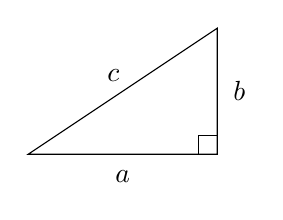
\begin{tikzpicture}[scale=0.8]
    \draw (0,0) -- (3,0) -- (3,2) -- cycle;
    \draw (2.7,0) -- (2.7,0.3) -- (3,0.3);
    \node at (1.5,-0.35) {$a$};
    \node at (3.35,1) {$b$};
    \node at (1.35,1.25) {$c$};
\end{tikzpicture}
\end{center}

\[
c^2=a^2+b^2
\]

\[
\text{Visual rearrangement can make the result appear evident.}
\]

\boardtakeaway{``Looks evident'' $\neq$ deductive proof}
\end{whiteboard}

The issue is not that the visual insight is worthless. The issue is
that a rigorous demonstration must establish every geometrical
claim on which the reasoning depends.

A diagram may invite us to see that a figure is a square, for
example, while a deductive proof must establish that fact from
previously accepted principles.

\newpage

\begin{whiteboard}
\textbf{FROM VISUAL INSIGHT TO DEMONSTRATION}

\[
\begin{array}{c}
\text{stated assumptions}\\
\downarrow\\
\text{lemma}\\
\downarrow\\
\text{lemma}\\
\downarrow\\
\text{theorem}
\end{array}
\]
\end{whiteboard}

% ============================================================
\section{The Euclidean Ideal}
% ============================================================

By the time of Euclid, the ideal of geometrical demonstration had
become much clearer.

The aim was to place the specifically geometrical assumptions at
the beginning and then construct chains in which later
propositions followed from those assumptions by necessity.

The Kneales note that Euclid himself does not always satisfy this
ideal perfectly. In the first proposition of the \textit{Elements},
for example, he relies upon an assumption concerning the
intersection of two circles without first stating a postulate from
which that result follows.

The significance of the example is methodological: if such an
unstated assumption were detected, the natural repair would be
to make the assumption explicit.

\begin{whiteboard}
\textbf{EUCLIDEAN IDEAL}

\[
\text{All special assumptions stated explicitly.}
\]

\vspace{0.4em}

\[
\begin{array}{c}
\text{hidden assumption}\\
\downarrow\\
\text{gap in demonstration}\\
\downarrow\\
\text{state an additional postulate}
\end{array}
\]

\boardtakeaway{A deductive system must expose its starting points.}
\end{whiteboard}

The history of geometry thus creates pressure toward explicit
axioms, explicit derivations, and explicit relations of
consequence.

% ============================================================
\section{What Geometry Encouraged Logicians to Notice}
% ============================================================

If Greek logical reflection developed partly from geometry, the
Kneales argue that several later features of Greek logic become
understandable.

\subsection{General Propositions}

Geometry is not fundamentally concerned with one unique
individual line or triangle.

When a geometer speaks of ``the line \(AB\),'' the object drawn
functions as a representative of any line satisfying the relevant
conditions.

\begin{whiteboard}
\textbf{1. GENERAL PROPOSITIONS}

\[
\text{``the line }AB\text{''}
\]

really functions as

\[
\text{any line satisfying the stated conditions.}
\]
\end{whiteboard}

\subsection{Necessary Universal Propositions}

Geometry also encourages a distinction between a universal
statement that merely happens to be true and one that is true by
necessity.

The propositions of geometry are supposed to belong to the
second class.

\begin{whiteboard}
\textbf{2. NECESSARY TRUTHS}

\[
\begin{array}{c}
\text{universally true by accident}\\
\neq\\
\text{universally true by necessity}
\end{array}
\]
\end{whiteboard}

\subsection{Definitions}

Definitions receive special importance.

Modern thinkers may regard some definitions as conventions about
the use of words. The Greeks did not generally understand
geometrical definitions in this merely conventional way.

A definition such as a characterization of a circle appeared to
state an important truth about circles themselves.

\begin{whiteboard}
\textbf{3. DEFINITIONS}

\[
\text{Greek view: definition}
\neq
\text{mere abbreviation}
\]

\[
\text{definition}
\longrightarrow
\text{tells us what the thing is}
\]
\end{whiteboard}

\subsection{Subsumption Under General Rules}

Finally, geometrical reasoning repeatedly involves applying a
general proposition to a more specific case.

This directs attention toward the relation between general kinds
and the particular or subordinate cases falling under them.

\begin{whiteboard}
\textbf{4. SUBSUMPTION}

\[
\text{specific case}
\quad\text{falls under}\quad
\text{general rule}
\]
\end{whiteboard}

The overall influence of geometry can therefore be summarized
compactly.

\begin{whiteboard}
\textbf{GEOMETRY ENCOURAGES ATTENTION TO}

\[
\begin{array}{ll}
1. & \text{General propositions} \\[0.3em]
2. & \text{Necessary truths} \\[0.3em]
3. & \text{Definitions} \\[0.3em]
4. & \text{Subsumption under general rules}
\end{array}
\]
\end{whiteboard}

These interests later become prominent in Aristotle.

% ============================================================
\section{Dialectic and Metaphysical Argument}
% ============================================================

Greek logic cannot be explained entirely through geometrical
demonstration.

A second major source is \textbf{dialectic}.

The word is historically important because it was an early
technical term for a kind of reasoning connected with
philosophical discussion. It is derived from a word associated
with discussion or conversation.

In Plato's middle-period dialogues, dialectical procedure often
takes the form of examining a hypothesis by tracing its
consequences.

If a hypothesis entails an unacceptable consequence, the
hypothesis is rejected.

\newpage

\begin{whiteboard}
\textbf{DIALECTIC}

\[
\boxed{
\text{Test a hypothesis by its consequences}
}
\]

\[
P\rightarrow Q
\]

\[
\neg Q
\]

\[
\therefore \neg P
\]

\[
\text{Hypothesis}
\rightarrow
\text{unacceptable consequence}
\rightarrow
\text{reject hypothesis}
\]
\end{whiteboard}

This is the characteristic structure of refutation
(\textit{elenchus}).

% ============================================================
\section{Zeno and Reductio ad Impossibile}
% ============================================================

The Kneales connect Platonic dialectic both with Socratic
refutation and with Zeno of Elea.

Zeno defended Parmenidean monism by drawing absurd
consequences from the supposition that plurality exists.

This form of reasoning is commonly described as
\textit{reductio ad impossibile}: a hypothesis is provisionally
accepted and then rejected because it produces an impossibility.

The method may itself have been encouraged by earlier
mathematical practice.

\begin{whiteboard}
\textbf{REDUCTIO AD IMPOSSIBILE}

\[
\begin{array}{c}
\text{Assume }P\\
\downarrow\\
\text{derive impossibility / contradiction}\\
\downarrow\\
\therefore \neg P
\end{array}
\]
\end{whiteboard}

The standard mathematical example discussed by the Kneales is
the proof of the incommensurability of the diagonal and side of a
square, expressed in modern terminology as the irrationality of
\(\sqrt{2}\).

% ============================================================
\section{Worked Example: The Irrationality of \(\sqrt{2}\)}
% ============================================================

Suppose, for the sake of argument, that \(\sqrt{2}\) is rational.

Then it can be expressed as a ratio

\[
\sqrt{2}=\frac{m}{n},
\]

where \(m\) and \(n\) are integers chosen with no common factor.

Squaring gives

\[
m^2=2n^2.
\]

Thus \(m^2\) is even, and therefore \(m\) is even.

Because the board is small, the demonstration is best performed
in two packets.

\begin{whiteboard}
\textbf{REDUCTIO: PACKET 1}

Assume

\[
\sqrt{2}=\frac{m}{n},
\]

where \(m,n\) are coprime.

Then

\[
m^2=2n^2.
\]

Therefore

\[
m^2\text{ is even}
\quad\Rightarrow\quad
m\text{ is even}.
\]

So let

\[
m=2k.
\]

\textit{Copy, then erase before Packet 2.}
\end{whiteboard}

Substituting \(m=2k\) into the equation gives

\[
(2k)^2=2n^2.
\]

Hence

\[
4k^2=2n^2
\]

and therefore

\[
n^2=2k^2.
\]

So \(n\) is also even.

But if both \(m\) and \(n\) are even, they share a common factor,
contrary to the original assumption that they were coprime.

The original hypothesis must therefore be false.

\begin{whiteboard}
\textbf{REDUCTIO: PACKET 2}

\[
m=2k
\]

so

\[
m^2=2n^2
\]

becomes

\[
(2k)^2=2n^2.
\]

Thus

\[
4k^2=2n^2
\]

and

\[
n^2=2k^2.
\]

Therefore

\[
n\text{ is even}.
\]

But then

\[
m\text{ even AND }n\text{ even},
\]

contradicting the assumption that \(m,n\) are coprime.

\[
\boxed{\therefore \sqrt{2}\text{ is irrational}}
\]
\end{whiteboard}

The logical structure is more important for us than the
mathematical result itself.

\begin{whiteboard}
\textbf{ABSTRACT FORM}

\[
\begin{array}{c}
\text{Assume }P\\
\downarrow\\
\text{contradiction}\\
\downarrow\\
\therefore \neg P
\end{array}
\]
\end{whiteboard}

This example helps connect the mathematical tradition of
demonstration with the philosophical tradition of dialectical
refutation.

% ============================================================
\section{Zenonian Reductio and the Socratic Elenchus}
% ============================================================

The Socratic method resembles Zeno's, but the Kneales point out
an important difference.

A strict Zenonian \textit{reductio ad impossibile} produces
incompatible consequences or an outright contradiction.

A Socratic refutation need not always reach a formal
contradiction. A hypothesis may instead be rejected because it
leads to a consequence independently regarded as false or
unacceptable.

The \textit{Meno}, for example, contains an argument against the
claim that virtue is teachable. If virtue were teachable, good men
would be expected successfully to teach it to their sons; the
failure of celebrated statesmen to do so is then used against the
original thesis.

\begin{whiteboard}
\textbf{TWO FORMS OF REFUTATION}

\[
\begin{array}{ll}
\textbf{Zenonian:}
&
P\rightarrow\text{contradiction}
\Rightarrow \neg P
\\[0.8em]
\textbf{Socratic:}
&
P\rightarrow Q,\quad Q\text{ false/unacceptable}
\Rightarrow \neg P
\end{array}
\]

\boardtakeaway{Both test a thesis through its consequences.}
\end{whiteboard}

% ============================================================
\section{Plato's Changing Use of ``Dialectic''}
% ============================================================

The word ``dialectic'' does not retain one fixed technical meaning
throughout Plato's writings.

In the middle-period dialogues, it is closely associated with the
testing of hypotheses through their consequences.

In Plato's later work, the name is transferred to the method of
\textbf{division and collection}.

Collection is less clearly explained, but division is illustrated
as a method for discovering definitions by repeatedly dividing a
general notion into alternatives.

\begin{whiteboard}
\textbf{PLATONIC ``DIALECTIC''}

\[
\begin{array}{ll}
\textbf{Middle period:}
&
\text{hypothesis}
\rightarrow
\text{consequences}
\rightarrow
\text{test}
\\[0.7em]
\textbf{Later period:}
&
\text{division + collection}
\rightarrow
\text{search for definition}
\end{array}
\]
\end{whiteboard}

In the \textit{Sophist}, Plato illustrates division through the
attempt to define an angler. A long classificatory tree narrows a
general concept by successive choices until the desired definition
is reached.

For a small whiteboard, only the selected path needs to be
written.

\begin{whiteboard}
\textbf{DIVISION: THE ANGLER}

\[
\begin{array}{c}
\text{technician}\\
\downarrow\\
\text{acquisitive}\\
\downarrow\\
\text{coercive}\\
\downarrow\\
\text{hunter}\\
\downarrow\\
\text{living things}\\
\downarrow\\
\text{water animals}\\
\downarrow\\
\text{fish}\\
\downarrow\\
\text{by day}\\
\downarrow\\
\text{with hooks}\\
\downarrow\\
\boxed{\text{angler}}
\end{array}
\]
\end{whiteboard}

The method may appear cumbersome, but it is historically
important. The Kneales argue that reflection upon it influenced
Aristotle's later development of syllogistic reasoning.

% ============================================================
\section{From Particular Arguments to Logical Principles}
% ============================================================

Plato also occasionally states logical principles explicitly in the
course of philosophical argument.

The Kneales illustrate the process by imagining a simple
exchange.

Suppose someone says:

\begin{center}
``Plato was a philosopher, so Plato was vague.''
\end{center}

If challenged, the speaker may supply an unstated general
premiss:

\begin{center}
``All philosophers are vague.''
\end{center}

The argument now becomes:

\[
\text{All philosophers are vague;}
\]

\[
\text{Plato is a philosopher;}
\]

\[
\therefore \text{Plato is vague.}
\]

\begin{whiteboard}
\textbf{MAKE THE PRINCIPLE EXPLICIT}

\[
\begin{array}{l}
\text{All philosophers are vague.}\\
\text{Plato is a philosopher.}\\
\hline
\therefore \text{Plato is vague.}
\end{array}
\]
\end{whiteboard}

We can then abstract still further from the subject matter.

\begin{whiteboard}
\textbf{ABSTRACT THE FORM}

\[
\begin{array}{l}
\text{Every }M\text{ is }L.\\
S\text{ is }M.\\
\hline
\therefore S\text{ is }L.
\end{array}
\]

\boardtakeaway{Logical form is independent of the particular subject matter.}
\end{whiteboard}

At this level, the principle no longer depends on whether we are
talking about philosophers, vagueness, Plato, or anything else.

Plato sometimes formulates principles of this kind, including a
version of the Law of Contradiction.

But he does so piecemeal, as particular arguments require them.
He does not assemble the principles into an organized formal
system.

\begin{whiteboard}
\[
\begin{array}{rcl}
\text{Plato: logical principles} & = & \text{YES}\\
\text{Plato: systematic formal logic} & = & \text{NO}
\end{array}
\]
\end{whiteboard}

This is one of the major differences between Plato and Aristotle.

% ============================================================
\section{Eristic, Sophistry, and the Problem of Verbal Form}
% ============================================================

A third source of early logical reflection comes from ordinary
argument, public disputation, and the investigation of fallacies.

An obvious first step toward logic is to notice that different
valid arguments seem to share recurring patterns.

But a danger immediately appears: two arguments may look
verbally similar while differing radically in validity.

The Kneales use a pair of examples to illustrate the problem.

\begin{whiteboard}
\textbf{ARGUMENT 1}

\[
\begin{array}{l}
\text{This is a pen.}\\
\text{This is blue.}\\
\hline
\therefore \text{This is a blue pen.}
\end{array}
\]
\end{whiteboard}

Compare:

\begin{whiteboard}
\textbf{ARGUMENT 2}

\[
\begin{array}{l}
\text{That dog is a father.}\\
\text{That dog is his.}\\
\hline
\therefore \text{That dog is his father.}
\end{array}
\]
\end{whiteboard}

The second argument resembles the first at the surface level of
words, but its premisses can be true while its conclusion is
false.

The similarity is therefore misleading.

\begin{whiteboard}
\[
\boxed{
\text{Same-looking words}
\neq
\text{same logical structure}
}
\]

\[
\text{Sophism}
=
\text{fallacious argument resembling a valid one}
\]
\end{whiteboard}

This is an important step in the discovery that logic cannot
simply classify strings of words by superficial grammatical
appearance.

% ============================================================
\section{Public Disputation}
% ============================================================

Plato and Aristotle provide evidence that formalized public
disputation had become a recognizable practice.

Typically, two people participate.

The \textbf{answerer} undertakes to maintain a thesis.

The \textbf{questioner} attempts to force the answerer to admit
consequences that are false, absurd, or otherwise unacceptable.

\newpage

\begin{whiteboard}
\textbf{PUBLIC DISPUTATION}

\[
\begin{array}{ll}
\textbf{Answerer:}
&
\text{maintain a thesis}
\\[0.6em]
\textbf{Questioner:}
&
\text{derive an unacceptable consequence}
\end{array}
\]
\end{whiteboard}

Such disputation could have several purposes.

It might contribute to philosophical investigation.

It might be practiced as intellectual amusement.

It might have practical applications in forensic or political
argument.

And the Kneales suggest that at least some apparently trivial
sophistical puzzles may have been connected with serious attempts
to distinguish valid principles from misleading verbal patterns.

\begin{whiteboard}
\textbf{USES OF DISPUTATION}

\[
\begin{array}{l}
\text{philosophical investigation}\\
\text{amusement}\\
\text{practical argument}\\
\text{logical investigation}
\end{array}
\]
\end{whiteboard}

% ============================================================
\section{The Megarian Route Toward Logic}
% ============================================================

The Kneales suggest that some pre-Aristotelian logical discussion
may have been centered in the Megarian school.

Its founder, Euclides of Megara, was associated both with the
Socratic tradition and with Eleatic philosophy.

The Megarians became famous for verbal controversy and were
sometimes called ``Eristics,'' but later Megarians such as
Diodorus Cronus and Philo displayed genuine logical
sophistication.

The Kneales therefore regard it as plausible that apparently
eristic disputation supplied material for serious logical
reflection.

\newpage

\begin{whiteboard}
\textbf{A SECOND HISTORICAL LINE}

\[
\begin{array}{c}
\text{debate / sophisms}\\
\downarrow\\
\text{reflection on argument}\\
\downarrow\\
\text{Megarian tradition}\\
\downarrow\\
\text{later Stoic logic}
\end{array}
\]
\end{whiteboard}

This development is significant because the history of logic does
not run through Aristotle alone.

% ============================================================
\section{Truth, Falsehood, and the Limits of Mere Words}
% ============================================================

The investigation of sophisms also raises deeper questions about
truth and falsehood.

The fragment known as the \textit{Dissoi Logoi} discusses cases
in which the same verbal expression can be true when uttered by
one person and false when uttered by another.

Consider the verbal form:

\begin{center}
``I am an initiate.''
\end{center}

It might be true when spoken by one person and false when spoken
by another.

\begin{whiteboard}
\textbf{SAME WORDS, DIFFERENT TRUTH VALUE}

\[
\text{``I am an initiate.''}
\]

\[
\begin{array}{rcl}
\text{spoken by A} &\longrightarrow& \text{TRUE}\\
\text{spoken by B} &\longrightarrow& \text{FALSE}
\end{array}
\]

\[
\boxed{
\text{Truth and falsity cannot belong to the verbal pattern alone.}
}
\]
\end{whiteboard}

This directs attention toward a question that will become central
in the philosophy of logic:

\begin{center}
\emph{What exactly is the thing that is true or false?}
\end{center}

\begin{whiteboard}
\[
\boxed{\text{WHAT IS TRUE OR FALSE?}}
\]
\end{whiteboard}

The Kneales suggest that reflection of this sort anticipates the
later Stoic distinction between an expression and what is
expressed by it.

% ============================================================
\section{Plato and the Philosophy of Logic}
% ============================================================

Although Plato does not construct a systematic formal logic, the
Kneales regard him as the first great thinker in the
\textbf{philosophy of logic}.

Three questions organize their discussion of his achievement.

\begin{whiteboard}
\textbf{PLATO: THREE QUESTIONS}

\[
\begin{array}{ll}
1. & \text{What can properly be TRUE or FALSE?}\\[0.4em]
2. & \text{What makes valid inference NECESSARY?}\\[0.4em]
3. & \text{What is the nature of DEFINITION?}
\end{array}
\]
\end{whiteboard}

These questions are not presented by Plato in precisely this
later form. The Kneales extract them from discussions in which
logical, metaphysical, and epistemological issues remain
interwoven.

% ============================================================
\section{Question One: What Is True or False?}
% ============================================================

In the \textit{Theaetetus}, Plato's discussion of knowledge leads
to the idea of true opinion.

But this raises a further problem: what is an opinion?

Plato sometimes describes thinking as an internal conversation of
the soul. Thought is a kind of silent discourse in which one asks,
answers, affirms, and denies.

This makes it natural to apply ``true'' and ``false'' either to
speech itself or to the corresponding act of thought.

In the \textit{Sophist}, Plato again associates thought and
discourse and treats complete discourse as involving at least a
noun and a verb.

The Kneales therefore detect two possible answers in Plato.

\begin{whiteboard}
\textbf{WHAT BEARS TRUTH OR FALSITY?}

Plato suggests:

\[
\begin{array}{ll}
1. & \text{sentence / discourse}\\[0.3em]
2. & \text{thought / judgement}
\end{array}
\]

Later Stoic alternative:

\[
3.\quad \text{proposition}
\]
\end{whiteboard}

Plato does not produce a fully explicit distinction among these
possibilities.

The third answer, associated with the proposition as something
distinct from both words and psychological acts, belongs to a
later stage of the history.

% ============================================================
\section{Question Two: What Makes Inference Necessary?}
% ============================================================

If valid inference consists in tracing necessary connexions, then
the previous question immediately leads to another:

\begin{center}
\emph{What are the things between which necessary connexions
hold?}
\end{center}

If truth belongs to sentences, one might suppose that necessity
is simply a relation between sentences.

If truth belongs to psychological acts, one might suppose that
necessity is a relation between thoughts.

The Kneales regard the second suggestion as especially
problematic, since people can think without reasoning validly.

Plato's characteristic answer instead appeals to the
\textbf{Forms}.

\begin{whiteboard}
\textbf{PLATO'S ANSWER}

\[
\boxed{
\text{Necessary connexions hold between Forms}
}
\]
\end{whiteboard}

For the logical point, we need only a limited account of the
Theory of Forms.

Forms are not ordinary physical things and are not merely private
ideas in a person's mind. They correspond at least partly to what
later philosophers call universals: common characters associated
with general terms.

Correct thinking follows the connexions among these Forms.

\begin{whiteboard}
\textbf{CORRECT THINKING}

\[
\begin{array}{c}
\text{Forms are connected in reality}\\
\downarrow\\
\text{thought follows those connexions}\\
\downarrow\\
\text{true discourse reflects reality}
\end{array}
\]
\end{whiteboard}

A sentence is true, on this interpretation, when the arrangement
expressed in discourse corresponds to the way realities are
actually connected.

\begin{whiteboard}
\boardtakeaway{For Plato, validity is grounded in how realities are connected, not merely in a verbal pattern.}
\end{whiteboard}

The Kneales note that Plato does not clearly handle every problem
generated by this position, including the distinction between
singular and general statements.

Nevertheless, the central historical idea is clear: logical
necessity is connected with an objective structure rather than
merely with arbitrary linguistic habits.

% ============================================================
\section{Being, Same, and Other}
% ============================================================

The \textit{Sophist} also contains a discussion of the unusually
general notions of \textbf{being}, \textbf{same}, and
\textbf{other}.

These terms do not operate in the same way as ordinary
classifying words such as ``red'' or ``kangaroo.''

They can enter into discourse about almost anything.

Plato's discussion helped direct attention toward terms that later
logical theories would have to treat differently from ordinary
predicates.

For the present lecture, however, the most important result is
that Plato helps remove two conceptual obstacles inherited from
earlier Greek philosophy: difficulties concerning negation and
difficulties concerning predication.

% ============================================================
\section{Negation and Predication}
% ============================================================

Earlier Greek thinkers had found something puzzling in speaking
of what ``is not.''

If not-being were simply nothing, then a negative assertion could
seem unintelligible.

A related confusion concerned statements of identity and
statements of predication.

The sentence

\[
A\text{ is }B
\]

does not always mean

\[
A=B.
\]

To say that Socrates is wise, for example, need not mean that
Socrates is identical with wisdom.

Plato's later work helps make room for meaningful negation and
non-identical predication.
\newpage

\begin{whiteboard}
\textbf{TWO OLD OBSTACLES}

\[
1.\quad \text{NEGATION: } A\text{ is not }B
\]

\[
2.\quad \text{PREDICATION: } A\text{ is }B
\]

but

\[
\boxed{\text{predication} \neq \text{identity}}
\]

and

\[
A\text{ is }B
\not\Rightarrow
A=B.
\]
\end{whiteboard}

The Kneales emphasize that removing these confusions was
important for the later development of logic.

\begin{whiteboard}
\[
\boxed{
\text{Plato clears conceptual ground for later logical theory.}
}
\]
\end{whiteboard}

% ============================================================
\section{Question Three: What Is a Definition?}
% ============================================================

Definitions are central throughout Plato's dialogues.

According to Aristotle, Plato inherited part of this concern from
Socrates' attempts to define ethical notions. Mathematical
practice probably supplied another important influence.

Plato treats definition as both \textbf{non-arbitrary} and
\textbf{informative}.

He recognizes that different languages can use different words
for the same thing. The choice of linguistic sign is therefore
conventional in an important sense.

But the object of definition is not, for Plato, merely the word.

Definition concerns the thing or Form to which the word refers.

\begin{whiteboard}
\textbf{WORD AND DEFINITION}

\[
\begin{array}{rcl}
\text{word}
&\longrightarrow&
\text{conventional sign}
\\[0.5em]
\text{definition}
&\longrightarrow&
\text{thing / Form}
\end{array}
\]
\end{whiteboard}

Thus the question

\begin{center}
``What is justice?''
\end{center}

is not merely the question

\begin{center}
``How do Greek speakers happen to use the word
\emph{justice}?''
\end{center}

It asks instead for the common nature that makes the relevant
things instances of justice.

This is the historical source of what is called a
\textbf{realistic theory of definition} or a
\textbf{real definition}.

\begin{whiteboard}
\textbf{REAL DEFINITION}

Not merely:

\[
\text{``How do we use this word?''}
\]

but:

\[
\boxed{\text{``What is the thing?''}}
\]

Examples:

\[
\text{What is justice?}
\]

\[
\text{What is colour?}
\]

\boardtakeaway{For Plato, definition is non-arbitrary and informative.}
\end{whiteboard}

This conception will strongly influence Aristotle even though
Aristotle rejects Plato's separate Forms.

% ============================================================
\section{How the Three Platonic Questions Fit Together}
% ============================================================

The Kneales' three questions are closely connected.

If logic concerns valid inference, validity involves necessary
connexion.

To understand necessary connexion, we must ask what sorts of
things are connected.

That question in turn requires us to ask what sort of thing can
be true or false.

And Plato's theory of definition supplies part of his answer to
how general thought connects with the structure of reality.
\newpage

\begin{whiteboard}
\textbf{PLATO'S LOGICAL PROBLEMS}

\[
\begin{array}{c}
\text{What is true or false?}\\
\downarrow\\
\text{What is connected in valid inference?}\\
\downarrow\\
\text{What structure does reality have?}\\
\downarrow\\
\text{What do definitions identify?}
\end{array}
\]
\end{whiteboard}

In Plato, therefore, logic has not yet separated cleanly from
metaphysics and epistemology.

That separation will itself be part of the later history.

% ============================================================
\section{Was There Logic Before Aristotle?}
% ============================================================

The evidence surveyed by the Kneales supports a qualified answer.

There was certainly substantial logical reflection before
Aristotle.

Greek geometers had reflected upon demonstration, axioms,
necessity, and consequence.

Zeno and Socrates had developed methods of refuting hypotheses
through their consequences.

Sophistical and eristic argument directed attention toward the
difference between genuinely valid structure and misleading
verbal appearance.

The Megarian tradition seems to have continued serious work on
logical puzzles.

Plato formulated some logical principles and investigated major
philosophical problems concerning truth, necessary connexion,
negation, predication, and definition.

\begin{whiteboard}
\textbf{BEFORE ARISTOTLE}

\[
\begin{array}{rcl}
\text{Geometry}
&\longrightarrow&
\text{demonstration}
\\[0.4em]
\text{Zeno / Socrates}
&\longrightarrow&
\text{refutation}
\\[0.4em]
\text{Sophists / Megarians}
&\longrightarrow&
\text{fallacy and argument}
\\[0.4em]
\text{Plato}
&\longrightarrow&
\text{truth, necessity, definition}
\end{array}
\]
\end{whiteboard}

But something crucial is still missing.

These investigations do not yet constitute a systematic formal
theory of inference.

Plato states logical principles as he requires them, but does not
organize them into a connected logical system.

The Kneales therefore preserve the magnitude of Aristotle's
achievement while rejecting the idea that logical reflection
began from nothing with Aristotle.

\begin{whiteboard}
\[
\boxed{
\begin{array}{c}
\text{Much logical reflection existed before Aristotle,}\\
\text{but no systematic formal logic yet.}
\end{array}
}
\]

\vspace{0.6em}

\[
\boxed{
\text{ARISTOTLE'S DECISIVE ACHIEVEMENT: SYSTEMATIZATION}
}
\]
\end{whiteboard}

% ============================================================
\section{Lecture Summary}
% ============================================================

The history traced in this chapter is not the story of a single
invention at a single moment.

Logical theory emerges gradually when Greeks begin reflecting
upon practices of proof and argument that already existed.

Geometry produces the ideal of necessary demonstration from
explicit starting points.

Metaphysical and Socratic dialectic develop the examination of
hypotheses through their consequences.

Sophistical and eristic disputes expose the danger of confusing
verbal similarity with valid logical form.

Plato then raises fundamental questions about truth and falsity,
necessary connexion, predication, negation, and definition.

These developments create much of the intellectual material from
which Aristotle will construct the first systematic theory of
formal logic.

\begin{whiteboard}
\textbf{SUMMARY}

\[
\begin{array}{c}
\text{Reasoning}\\
\downarrow\\
\text{reflection on validity}\\
\downarrow\\
\text{logic}
\end{array}
\]

\vspace{0.5em}

\[
\begin{array}{rcl}
\text{Geometry}
&\rightarrow&
\text{demonstration / consequence}
\\[0.3em]
\text{Dialectic}
&\rightarrow&
\text{hypothesis / refutation}
\\[0.3em]
\text{Sophistry}
&\rightarrow&
\text{validity vs.\ verbal appearance}
\\[0.3em]
\text{Plato}
&\rightarrow&
\text{truth / necessity / definition}
\end{array}
\]

\vspace{0.6em}

\boardtakeaway{Pre-Aristotelian Greeks supplied the problems and methods; Aristotle supplied systematic formal theory.}
\end{whiteboard}

\end{document}